\documentclass[journal]{vgtc}                % final (journal style)
%\documentclass[review,journal]{vgtc}         % review (journal style)
%\documentclass[widereview]{vgtc}             % wide-spaced review
%\documentclass[preprint,journal]{vgtc}       % preprint (journal style)

%% Uncomment one of the lines above depending on where your paper is
%% in the conference process. ``review'' and ``widereview'' are for review
%% submission, ``preprint'' is for pre-publication, and the final version
%% doesn't use a specific qualifier.

%% These few lines make a distinction between latex and pdflatex calls and they
%% bring in essential packages for graphics and font handling.
%% Note that due to the \DeclareGraphicsExtensions{} call it is no longer necessary
%% to provide the the path and extension of a graphics file:
%% 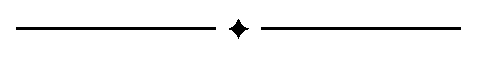
\includegraphics{diamondrule} is completely sufficient.
%%
\ifpdf%                                % if we use pdflatex
  \pdfoutput=1\relax                   % create PDFs from pdfLaTeX
  \pdfcompresslevel=9                  % PDF Compression
  \pdfoptionpdfminorversion=7          % create PDF 1.7
  \ExecuteOptions{pdftex}
  \usepackage{graphicx}                % allow us to embed graphics files
  \DeclareGraphicsExtensions{.pdf,.png,.jpg,.jpeg} % for pdflatex we expect .pdf, .png, or .jpg files
\else%                                 % else we use pure latex
  \ExecuteOptions{dvips}
  \usepackage{graphicx}                % allow us to embed graphics files
  \DeclareGraphicsExtensions{.eps}     % for pure latex we expect eps files
\fi%

%% it is recomended to use ``\autoref{sec:bla}'' instead of ``Fig.~\ref{sec:bla}''
\graphicspath{{figures/}{pictures/}{images/}{./}} % where to search for the images

\usepackage{microtype}                 % use micro-typography (slightly more compact, better to read)
\PassOptionsToPackage{warn}{textcomp}  % to address font issues with \textrightarrow
\usepackage{textcomp}                  % use better special symbols
\usepackage{mathptmx}                  % use matching math font
\usepackage{times}                     % we use Times as the main font
\renewcommand*\ttdefault{txtt}         % a nicer typewriter font
\usepackage{cite}
\usepackage{amsmath}
%% If you are submitting a paper to a conference for review with a double
%% blind reviewing process, please replace the value ``0'' below with your
%% OnlineID. Otherwise, you may safely leave it at ``0''.
\onlineid{0}

%% declare the category of your paper, only shown in review mode
\vgtccategory{Research}

%% Paper title - 1 pt for descriptive title
\title{Automatic Feature Detection in Hardware Performance Metric Data based on User Feedback}

%% This is how authors are specified in the journal style

%% indicate IEEE Member or Student Member in form indicated below
%% 1 pt for name
\author{Sayef Azad Sakin}
\authorfooter{
%% insert punctuation at end of each item
\item
Sayef Azad Sakin is a graduate student at the University of Arizona. E-mail:sayefsakin@email.arizona.edu.
}

%other entries to be set up for journal
%\shortauthortitle{Firstauthor \MakeLowercase{\textit{et al.}}: Paper Title}

%% Abstract section - 5 pts
\abstract{
Understanding large scale runtime system behavior becomes harder as the hardware performance metric data grows significantly over time. Identifying
relationship within different performance metric could be accessory to assessing and evaluating these data. The Traveler project provides an integrated
visualization system for visualizing performance metric data. It uses OTF2 execution traces and present them over several interactive views like - Gantt
view, Utilization view, Time series view etc. Highlighting key features from these views is crucial to artifact detection and optimization of a runtime system.
Therefore, providing prediction of different features in advance will be helpful for user to browse, lookup, and identify them. Also the prediction could be
useful for any backend caching mechanism to load data in advance, hence improving user interactivity. In this project, an automated learning based feature
prediction model has been proposed for analysing temporal performance metric data labeled by the user and providing prediction of
interesting features for any future performance data. A dedicated python class has been developed for the Traveler platform to provide the feature prediction,
which could be utilized by any backend data model or directly integrated as a module with the frontend controller.
} % end of abstract

%% Keywords that describe your work. Will show as 'Index Terms' in journal
%% please capitalize first letter and insert punctuation after last keyword
%\keywords{Radiosity, global illumination, constant time}

%% ACM Computing Classification System (CCS). 
%% See <http://www.acm.org/class/1998/> for details.
%% The ``\CCScat'' command takes four arguments.

%\CCScatlist{ % not used in journal version
% \CCScat{K.6.1}{Management of Computing and Information Systems}%
%{Project and People Management}{Life Cycle};
% \CCScat{K.7.m}{The Computing Profession}{Miscellaneous}{Ethics}
%}

%% Uncomment below to include a teaser figure.
%   \teaser{
%   \centering
%   \includegraphics[width=16cm]{CypressView}
%   \caption{In the Clouds: Vancouver from Cypress Mountain.}
%  }

%% Uncomment below to disable the manuscript note
%\renewcommand{\manuscriptnotetxt}{}

%% Copyright space is enabled by default as required by guidelines.
%% It is disabled by the 'review' option or via the following command:
% \nocopyrightspace

\vgtcinsertpkg

%%%%%%%%%%%%%%%%%%%%%%%%%%%%%%%%%%%%%%%%%%%%%%%%%%%%%%%%%%%%%%%%
%%%%%%%%%%%%%%%%%%%%%% START OF THE PAPER %%%%%%%%%%%%%%%%%%%%%%
%%%%%%%%%%%%%%%%%%%%%%%%%%%%%%%%%%%%%%%%%%%%%%%%%%%%%%%%%%%%%%%%%

\begin{document}

%% The ``\maketitle'' command must be the first command after the
%% ``\begin{document}'' command. It prepares and prints the title block.

%% the only exception to this rule is the \firstsection command
%\firstsection{Introduction} % or "Motivation"

\maketitle

\section{Overview}
\label{sec:overview}
Large-scale parallel applications have become the backbone of a wide variety of scientific and technological research\cite{ashby2010opportunities,
hoisie2012ascr}. Deciphering features from the runtime system of these appications as well as optimizing them is a significant and largely unsolved problem\cite{daly2011tools}. Optimizing resources related to time-oriented process scheduling is essential for productivity. Time series visualization provides a
practical medium for exploratory visual data analysis of these parallel systems\cite{aigner2011visualization}. Typically, high-end scientific
simulations require time consuming and intensive operations, incurring massive temporal dataset to decipher. Interactive visual data exploration
of these massive temporal dataset is becoming increasingly challenging due to the rapid generation of data, in the order of terabytes or petabytes.
Therefore, an automated feature recommender system of a temporal dataset is essential for exploratory data analysis. It will also give clues on how different
hardware metrics change over time, which could be valuable information for scientists required to run, analyze, and tweak high-end time consuming simulations.
\par
Phylanx\cite{tohid2018asynchronous} is a general purpose computation system of distributed arrays to enhance operations over large-scale distributed system. It
is an actively-developed system to provide the benefits of distributed resources for data scientists. Phylanx first translates the code into PhySL, an intermediate
representation in a domain-specific, functional language. The function calls, control flow operations, data operations, and blocks found in the PhySL
representation are referred to as primitives. These primitives are translated to tasks in the HPX, a C++ standard library and asynchronous tasking runtime.
The dependencies of each primitive are the arguments it needs to execute (which may be other primitives), data access operations, or any other constraints on
variables the primitive uses. Temporal execution information of Phylanx is printed on a trace file and visualized using Traveler.
\par
The Traveler \cite{Traveler2019} is an integrated graph visualization system for asynchronous multi-task execution. It uses
OTF2\cite{otf2_developer_community_2019_3356709} \cite{knupfer2012score} trace data generated from Phylanx execution, parse them, and represent them in
different interactive views\textemdash Gantt view, Utilization view, Tree view, and Time series view, etc. Due to the massive number of temporal data, the
loading time of these views becomes slower and conspicuous lagging becomes apparent during interactive inspection over these views. The goal of my project is
the identification and discovery of interesting features\textemdash like cache overflow, unnecessary memory overhead, CPU exhaustion or starvation,
etc .\textemdash from the temporal dataset of hardware performance metric. In the aim of achieving this goal, an automated learning based recommender system
has been developed to predict and recommend interesting features which will be useful for further analysis of the runtime system (the trace data it is used
to learn from). The contributions of my project are summarized as follows:
\begin{itemize}
    \item Recommender Engine modeling - The dual space model (DSM)\cite{huang2018optimization} proposed by Huang et al. has been adapted to design a
    recommender engine.
    \item Feature abstraction - Temporal data of a performance metric from different hardware locations have been converted into individual input features for
    the recommender engine.
    \item Data adapter - An intermediate parser has been designed to receive data from the Traveler platform to the recommender engine, parse them and
    sent back through a convenient interface.
    \item Performance evaluation - An elementary performance evaluation has been conducted to assess the practicality and feasibility of the designed
    recommender model.
\end{itemize}


\section{Related Works}
\label{sec:background}
Large-scale web-based pan/zoom visualizations developed by Tao et al.\cite{tao2019kyrix} is more relevant to my project. Their technique was mostly to
predict next pan/zoom location which required less intensive learning based techniques. They developed a declarative language for easy specification of user
behavior and data management model. Battle et al.\cite{battle2019role} did thorough investigation of explorative data analysis by showing comparison between
latency, task complexity, and user performance. An earlier work\cite{battle2014dynamic} from the same author analysed different statistical characteristics
(e.g. histogram) among multiple user interactions over temporal dataset. They also proposed a general purpose tool, \emph{ForeCache}\cite{battle2016dynamic},
for exploratory browsing of large dataset. By learning first from the user's movements, they prefetched the data using different statistical data
characteristics to find similarity to the user's past behavior. Their data model and the prediction engine design has been considered a baseline for
measurement in visual data exploratory domain. Liu et al.\cite{liu2013immens} proposed a specialized data structure called multivariate data tiles for
dynamic loading and pre-processing of data. They also synthesis the data for better representation and processing parallelization. Huang el al.
\cite{huang2018optimization} \cite{huang2019aideme} used active learning framework to leverage the subspatial context and conjunctive context of database queries. Their
developed
dual space model algorithm able to bypass the slow convergence problem of active learning techniques. In my project, most of their proposed mechanisms have
been adapted due to the high similarity of the problem domain and use cases. \emph{Skyrec}\cite{liu2019improvement} of Liu et al. used query session summary
method to ease-up the query recommendations. They also developed a frontend interface named \emph{SkyServer Surfliner} for interactive recommendation.

\section{Technical Details}
\label{sec:technical}
Technical details goes here

\section{Evaluation}
\label{sec:evaluation}
How did you evaluate.
%The evaluation is conducted in two phases. In the first phase, a short presentation of this project was given in front of some students and their feedback was
%collected over an online form. In the second phase, an email was sent to the Phylanx developers, containing some screenshots of the visualization and their
%feedback was collected over email. Both of these evaluation phases are described in the following two subsections.
%%
%%
%\subsection{Non-expert Feedback}
%A short presentation about this project was delivered with some visual demonstration (with screenshots) in front of a set of participants. The participants of
%my presentation are 10 graduate students from the department of computer science, applied mathematics, lunar \& planetary lab of University of Arizona. During
%the presentation, I covered both the backend data handling and frontend visual design and representation methodologies after providing some background
%knowledge of Phylanx and traveler-integrated project. With the help of the course instructor, an online form was presented to the participants and feedback
%was collected from each of them. The participants were asked about what they think the strength of my project and how it could be improved.
%\par
%Most of the participants found the visualization intuitive as it works with temporal data and presents that in conventional way. Some of them liked the
%juxtaposed views and interactive features over multiple views like zoom in/out, mouse hover, etc. Two participants also commented that, my visualization
%makes it easier and clear to find points where CPU utilization cycles are changing which will help in debugging. There is also one participant who couldn't
%understand my visualization as the participant mentioned the presentation wasn't clear enough.
%\par
%The suggestions given by the participants were very informative and helpful toward the future direction of my project. Most of the participants suggested to
%use color encoding based on some properties to increase the identification of individual line. One mentioned to use pop-out functionality to highlight or
%isolate data points. Some pointed out to use clustering methods for different location to make the visualization less cluttered. On participant advised to
%use binary search tree during data bundling instead of the interval tree.
%%
%%
%\subsection{Expert Evaluation}
%Since I worked with OTF2 trace data generated from Phylanx execution on parallel machines, I reached out to Phylanx team members, via email, for their feedback
%on how my visualization can augment into their debugging and artifact isolation process. I included several screenshots of my visualization with relevant
%description of the functionalities. Two of the principal investigators of Phylanx replied to that email and commented on the visualization.
%\par Both of the principal investigators praised the newly developed line chart, after some back-and-forth emailing with the
%functionality description. One of them pointed out that, the core design is useful to represent the metric PAPI\_L1\_DCM (level 1 data cache misses), while
%in my design, I used the metric PAPI\_TOT\_CYC (cpu cycle). Also a bug on the trace data\textemdash which prints the same metric values for consecutive
%enter/leave events\textemdash was manifested and acknowledged by the investigators.
%%
%%
%\subsection{Discussion}
%It was clear from the evaluation that the newly developed line chart in association with other views (Gantt view, Utilization view) augments in understanding
%of the trace data. Though only one metric is used, the core design of the visualization is useful to represent different hardware performance metric values.
%It also becomes intuitive to track down primitive and its related metric values because of the juxtaposed view design. Small tweaking on the gantt view, like
%highlighting similar intervals with same GUID and primitive name helped to instrument the dependencies among them.
%\par Several interactive features like zoom in/out, panning increase the readability of the line chart which makes the frontend more effective for
%representing traces from longer running program executions. Also the usage of interval tree on the backend with some performance tweaking on histogram
%calculation make it more adaptable to higher number of input trace data. These design choices make the visualization comparatively more scalable with respect
%to the previous implementation of the traveler project. Though the visual design and the backend implementation hasn't ready for adapting into other parallel
%system (than Phylanx), it gives a proper indication on how to do so\textemdash with convenient API design and backend data parsing would easily make it
%adaptable to other distributed programs.
%\subsection{Limitations}
%The target population (domain expert) for this project is really small\textemdash only limited to the team members of Phylanx. Since the traveler project is an
%actively developed project, it has some complex procedures on live deployment and dependency on over several other modules to
%become ready. Because of this, a live demo for the limited number of Phylanx experts was not possible during the evaluation process. Though it could be done
%with remote desktop sharing methods, it will not be convenient for the participants. Again, while collecting feedback with email, the description of the
%views was not clear and concise. A formatted description with related questionnaries and prerecorded video demo would make the evaluation over the email more
%convenient.
%\subsection{Future Evaluations}
%In future, more formatted evaluation will be conducted through exhaustive feedback procedures to make the visualization more effective for the Phylanx
%members. A live demo will be prepared by deploying the project and make it accessible for the participants. A set of predefined questions will be prepared
%for the evaluation process. The questions will be presented and feedback will be collected via online forms, so that the participants can submit the forms in
%their convenient time just by testing the live demo. Relevant logging system will be maintained to track down the interaction of the participants over the
%visualizations.

\section{Future Direction}
\label{sec:future}
There are several limitations and pending modifications exist in my project which will be a good starting point for further work in the future. First of all,
an extensive user data collection should be conducted to make the prediction engine more valid and practically representative. A seperate
script can be used to either get new user input or incorporate old user data for the recommender system. Secondly, the implemented dual space model only
initiates with the labeled user data once prior to the iterations. The original DSM implementation used a probabilty function to choose between labeled
user data and DSM predicted data in successive iterations as the input for the consecutive iterations. This uncertainty sampling technique is necessary to
reduce the version space, the space of all configuration of the classification model consistent with the labeled data, for enabling an approximation of the
optimal algorithm. Thirdly, The increased number of hardware locality in a large-scale systems can easily exhaust the feature dimension. Therefore,
factorization techniques should be adapted to reduce the high-dimensional data space to a lower-dimensional spaces. Lastly, a comprehensive user study should
be conducted to evaluate the performance of the recommender system. Also, how well the prediction aligned with real life hardware artifacts can also be tracked
and used to create a validation dataset for the system.


\section{Conclusion}
\label{sec:summary}
Learning based interactive database exploration is an ongoing research problem in scientific community. I started working on this project to make the data
exploration of Traveler more interactive and convenient for the user based on an active learning based prediction technique. After doing some literature
study, I've came to know about state-of-the art works like \emph{ForeCahce}\cite{battle2016dynamic}, \emph{Kyrix}\cite{tao2019kyrix},
\emph{Skyrec}\cite{liu2019improvement}, \emph{DSM}\cite{huang2018optimization}, etc. I designed a parser to fetch live formatted OTF2 performance data from
the Traveler. To make the data labeling easier, a separate script is written to label the dataset and present to the recommender model. The parsed data is
formated accordingly to the feature abstraction described in Section\ref{sec:technical}. Then by following the DSM algorithm, the basic classifier engine has
been developed with slight tweaking according to the domain needs. A conveninent interface has been provided to make prediction feedback available towards
the Traveler system. Lastly, A priliminary performance evaluation has been conducted to assess the engine on how well it predicted based on the labelling
provided by the user. A comprehensive report has been created and necessary description provided in this report with the insights learned through this
project.

%\bibliographystyle{abbrv}
\bibliographystyle{abbrv-doi-hyperref}
%%use following if all content of bibtex file should be shown
%\nocite{*}
\bibliography{report}
\end{document}

